\documentclass[twoside,11pt]{article}

% JMLR style
\usepackage{jmlr2e}

% Make links clickable and visible
\hypersetup{
    colorlinks=true,
    linkcolor=blue,
    citecolor=blue,
    urlcolor=blue
}

\usepackage{amsmath,amssymb,amsfonts}
\usepackage{graphicx}
\usepackage{booktabs}
\usepackage{algorithm}
\usepackage{algpseudocode}
\usepackage{hyperref}
\usepackage{xcolor}
\usepackage{tikz}
\usetikzlibrary{shapes,arrows,positioning,calc}
\usepackage{pifont}
\newcommand{\cmark}{\ding{51}}
\newcommand{\xmark}{\ding{55}}

% Custom commands
\newcommand{\bem}{\textsc{BEM}}
\newcommand{\alfm}{\textsc{ALFM}}
\newcommand{\R}{\mathbb{R}}
\newcommand{\E}{\mathbb{E}}
\newcommand{\N}{\mathcal{N}}
\newcommand{\qed}{\hfill\ensuremath{\square}}

% Heading arguments are {short title}{short author}
\ShortHeadings{ALFM-BEM}{Ahmann}
\firstpageno{1}

\title{ALFM-BEM: Bidirectional Experience Memory for\\Continuous Learning in Foundation Model Deployments}

\author{\name David Ahmann \email dahmann@lumyn.cc \\
       \addr Independent Researcher\\
       Toronto, Canada}

\editor{Action Editor}

\begin{document}

\maketitle

\begin{abstract}
Foundation models are deployed frozen, creating a fundamental gap: they cannot learn from deployment experiences. We introduce ALFM-BEM (Adaptive Latent Feedback Model with Bidirectional Experience Memory), a unified wrapper architecture that enables continuous learning without modifying backbone weights. The central abstraction is \emph{Bidirectional Experience Memory} (BEM), a single memory structure where experiences live on a continuous outcome spectrum from failure to success. BEM naturally provides: (1) risk signals from failure similarity, (2) success patterns for retrieval-augmented reasoning, and (3) out-of-distribution detection as an emergent property of coverage. We extend the Consensus Engine with a fourth action---\textsc{Query}---that transforms passive abstention into active learning by requesting specific information when operating outside the experience distribution. Bounded adapters trained via experience replay enable continual improvement with provable stability guarantees. Experiments on synthetic deployment scenarios demonstrate effective failure retrieval (F1 $>$ 0.99), strong OOD detection capability (AUC $\approx$ 1.0 for clustered patterns), and bounded parameter drift under continuous training. ALFM-BEM is backbone-agnostic and provides deployment infrastructure for frozen models while the fundamental architecture limitations they exhibit remain unsolved.
\end{abstract}

\section{Introduction}
\label{sec:intro}

The deployment of foundation models reveals a structural tension: these models are designed for generalization across tasks but lack mechanisms for adaptation to specific deployment contexts. A model that exhibits specific failure modes today will repeat them tomorrow. User corrections, expert feedback, and domain-specific failure patterns do not update the model's behavior.

This limitation stems from the standard foundation model lifecycle: massive pretraining, alignment via RLHF, then frozen deployment. While this paradigm enables broad capability, it creates three gaps:

\textbf{Gap 1: No memory of past failures.} When a model makes an error, nothing inside records this failure. The same error pattern recurs whenever similar inputs arise.

\textbf{Gap 2: No calibrated self-doubt.} Foundation models produce confident outputs even when operating outside their reliable capability boundaries.

\textbf{Gap 3: No safe continual learning.} Standard fine-tuning risks catastrophic forgetting and is impractical for per-tenant customization.

Recent discourse among AI researchers has emphasized that while current scaling continues to improve models on benchmarks, something fundamental is missing for true ``learning machines'' that can acquire knowledge on the job. Large language models cannot learn from their deployment experiences~\cite{Brown2020,Touvron2023}; they repeat the same mistakes indefinitely. The disconnect between evaluation performance and real-world economic impact suggests that existing architectures may be reaching the limits of what static deployment can achieve.

We propose ALFM-BEM, a wrapper architecture that addresses these gaps without modifying backbone weights. Our key insight is that the three gaps can be addressed by a \emph{single unified abstraction}: Bidirectional Experience Memory (BEM).

\subsection{Contributions}

\begin{enumerate}
    \item We introduce \textbf{Bidirectional Experience Memory (BEM)}, a unified memory architecture where experiences exist on a continuous outcome spectrum. BEM provides risk signals, success patterns, and OOD detection as properties of a single structure---not as separate bolted-on components.
    
    \item We extend the Consensus Engine with a \textbf{Query action} that transforms passive abstention into active learning by requesting specific information when the system operates outside its experience distribution.
    
    \item We present \textbf{bounded adapters with experience replay} that enable continuous improvement from deployment outcomes while maintaining provable stability guarantees.
    
    \item We demonstrate experimentally that BEM achieves effective failure retrieval, OOD detection, and stable continuous learning on synthetic deployment scenarios.
\end{enumerate}

\section{Related Work}
\label{sec:related}

\textbf{Memory-Augmented Networks.} Neural Turing Machines~\cite{Graves2014}, Differentiable Neural Computers~\cite{Graves2016}, and Memory Networks~\cite{Weston2015} introduced differentiable memory for neural networks. Recent work extends attention with retrieval~\cite{Wu2022,Borgeaud2022}. MemGPT~\cite{Packer2023} implements virtual context management for extended conversations. These approaches store \emph{information}; BEM stores \emph{experiences with outcomes}, enabling learning from deployment. The key distinction: RAG retrieves facts, BEM retrieves what worked and what failed.

\textbf{Selective Prediction and Calibration.} Selective prediction~\cite{Chow1970,ElYaniv2010,Geifman2017} allows models to abstain when uncertain. Modern neural networks are poorly calibrated~\cite{Guo2017}; learning to defer~\cite{Madras2018} routes difficult examples to experts. Our Consensus Engine extends this with the Query action---not just abstaining but actively requesting what would help.

\textbf{Out-of-Distribution Detection.} Detecting when inputs fall outside the training distribution is critical for safe deployment. Baseline methods use softmax confidence~\cite{Hendrycks2017}; energy-based approaches~\cite{Liu2020} improve discrimination. BEM's coverage signal provides OOD detection as an emergent property---low coverage indicates operation outside the experience distribution.

\textbf{Continual Learning.} Approaches include regularization~\cite{Kirkpatrick2017}, replay buffers~\cite{Rolnick2019}, and architectural methods~\cite{Rusu2016}. Parameter-efficient methods like LoRA~\cite{Hu2022} and adapters~\cite{Houlsby2019} enable adaptation without full retraining. ALFM-BEM combines bounded adapters with experience replay from BEM, providing continual improvement with provable stability.

\textbf{Contrastive Representation Learning.} Contrastive methods~\cite{Chen2020,Radford2021} learn representations by pulling similar examples together and pushing dissimilar ones apart. BEM's projection layer uses contrastive learning to create an experience-separable space where failures cluster distinctly from successes.

\textbf{AI Safety.} Constitutional AI~\cite{Bai2022} and guardrails~\cite{Rebedea2023} encode static constraints. BEM complements these with dynamic, learned constraints from deployment experience---the system learns which contexts lead to failures.

\textbf{Retrieval-Augmented Generation.} RAG~\cite{Lewis2020} augments models with retrieved documents. BEM differs fundamentally: it stores experiences (context + outcome), not information. This enables learning from deployment: the system knows not just what to retrieve, but what worked and what failed in similar contexts.

\section{Architecture}
\label{sec:arch}

ALFM-BEM wraps a frozen backbone $\mathcal{M}$ with four components connected by a closed experience loop. Figure~\ref{fig:arch} illustrates the architecture.

\begin{figure}[t]
    \centering
    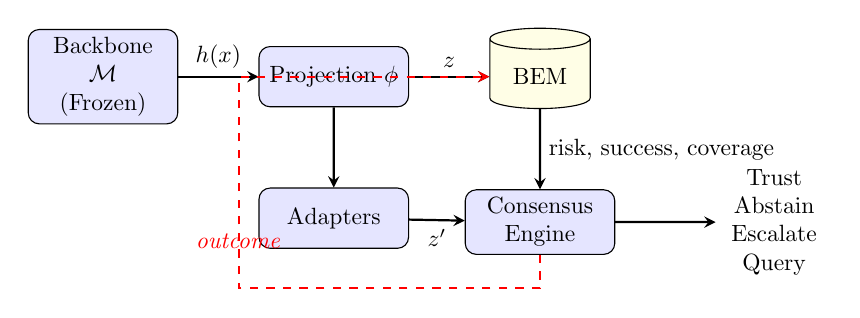
\begin{tikzpicture}[node distance=1.2cm, >=stealth, scale=0.85, transform shape]
        \tikzstyle{block} = [rectangle, draw, fill=blue!10, text width=2cm, text centered, rounded corners, minimum height=0.9cm]
        \tikzstyle{mem} = [cylinder, shape border rotate=90, draw, fill=yellow!10, aspect=0.3, minimum height=1.2cm, minimum width=1.5cm]
        \tikzstyle{line} = [draw, ->, thick]
        
        \node [block] (backbone) {Backbone $\mathcal{M}$\\(Frozen)};
        \node [block, right=of backbone] (proj) {Projection $\phi$};
        \node [mem, right=of proj] (bem) {BEM};
        \node [block, below=of proj] (adapter) {Adapters};
        \node [block, below=of bem] (consensus) {Consensus Engine};
        \node [right=1.5cm of consensus, text width=1.5cm, align=center] (actions) {Trust\\Abstain\\Escalate\\Query};
        
        \path [line] (backbone) -- node[above] {$h(x)$} (proj);
        \path [line] (proj) -- node[above] {$z$} (bem);
        \path [line] (bem) -- node[right] {risk, success, coverage} (consensus);
        \path [line] (proj) -- (adapter);
        \path [line] (adapter) -- node[below] {$z'$} (consensus);
        \path [line] (consensus) -- (actions);
        
        % Experience loop - goes DOWN from consensus, LEFT, then UP to BEM
        \draw[->, thick, dashed, red] (consensus.south) -- ++(0,-0.5) -| ++(-4.5,0) |- node[pos=0.15, below, red] {\textit{outcome}} (bem.west);
    \end{tikzpicture}
    \caption{ALFM-BEM architecture. The backbone remains frozen. The projection layer maps hidden states to experience-separable space. BEM provides risk/success/coverage signals. The Consensus Engine decides actions. The dashed red line shows the experience loop: outcomes feed back into BEM, closing the learning cycle.}
    \label{fig:arch}
\end{figure}

\textbf{Contrastive Dataset Construction.} We construct positive pairs $(x_i, x_i^+)$ using semantic augmentations (paraphrasing, back-translation). Negative pairs $(x_i, x_j^-)$ are mined from: (a) random batch negatives, and (b) \emph{hard negatives}---contexts that are semantically close but have divergent outcomes (success vs. failure). Specifically, we mine hard negatives by selecting successful contexts $x_j$ such that $\mathrm{sim}(\phi(x_i), \phi(x_j)) > \tau$ but $y_i \neq y_j$. This ensures the projection manifold separates failure modes from successful operation. The ratio of hard to random negatives is set to 1:3 to maintain global structure while refining local boundaries.

\subsection{Bidirectional Experience Memory (BEM)}
\label{sec:bem}

BEM is the central abstraction that unifies failure memory, success memory, and OOD detection into a single coherent structure.





\textbf{Definition 3.1 (Experience).} An experience $e$ is a tuple $(z_e, o_e, t_e, d_e, m_e)$ where $z_e \in \R^d$ is the projected embedding, $o_e \in [-1, 1]$ is the continuous outcome (negative = failure, positive = success), $t_e$ is tenant ID, $d_e$ is domain ID, and $m_e$ is metadata.

\textbf{Key Design Principle.} Experiences are points in embedding space with continuous outcome labels. There is no hard boundary between ``failure memory'' and ``success memory''---they are two views of the same structure.

\textbf{Definition 3.2 (Risk Signal).} Given query embedding $z$ and threshold $\theta$:
\begin{equation}
    s_{\text{risk}}(z) = 1 - \prod_{e \in \mathcal{N}(z,\theta), o_e < -0.3} \left(1 - \alpha \cdot \text{sim}(z, z_e) \cdot |o_e|\right)
\end{equation}
where $\mathcal{N}(z, \theta) = \{e : \text{sim}(z, z_e) > \theta\}$ and $\alpha$ is sensitivity. This noisy-OR aggregation models the probability that at least one relevant failure mode is active.

\textbf{Definition 3.3 (Success Signal).} Analogously:
\begin{equation}
    s_{\text{success}}(z) = \frac{1}{|\mathcal{N}^+(z,\theta)|} \sum_{e \in \mathcal{N}^+(z,\theta)} \text{sim}(z, z_e) \cdot o_e
\end{equation}
where $\mathcal{N}^+(z, \theta) = \{e \in \mathcal{N}(z,\theta) : o_e > 0.3\}$.

\textbf{Definition 3.4 (Coverage Signal).} The coverage signal measures how well $z$ is represented in the experience distribution---an emergent property, not a separate detector. We use kernel density estimation (KDE) over cosine similarities:
\begin{equation}
    s_{\text{cov}}(z) = \text{clip}\left(\kappa \cdot \frac{1}{|\mathcal{E}|} \sum_{e \in \mathcal{E}} \exp\left(-\frac{(1 - \text{sim}(z, z_e))^2}{2h^2}\right), 0, 1\right)
\end{equation}
where $h$ is the KDE bandwidth (we use $h = 0.3$) and $\kappa$ is a scaling constant. This KDE formulation captures local density in experience space. For clustered patterns, KDE coverage achieves near-perfect OOD detection (AUC $\approx$ 1.0) because novel clusters have no nearby experiences. Low coverage indicates out-of-distribution operation.

\subsection{Consensus Engine with Query Action}
\label{sec:consensus}

The Consensus Engine arbitrates between a Semantic Agent (BEM signals) and a Heuristic Agent (deterministic rules) to produce one of four actions.

The \textbf{Heuristic Agent} enforces hard constraints using: (1) \textbf{Regex Matchers} for PII and banned patterns; (2) \textbf{Symbolic Verifiers} for arithmetic and date logic; and (3) \textbf{Constraint Checkers} for JSON schema compliance. These rules provide a safety floor that overrides semantic signals.

\textbf{Actions:}
\begin{itemize}
    \item \textsc{Trust}: Use backbone output
    \item \textsc{Abstain}: Decline with explanation
    \item \textsc{Escalate}: Route to human review
    \item \textsc{Query}: Request specific information (new)
\end{itemize}

The Query action is the key extension. When coverage is low, instead of passively abstaining, the system identifies what type of information would help:
\begin{itemize}
    \item \textsc{Clarification}: Input is ambiguous
    \item \textsc{Precedent}: No similar successful cases
    \item \textsc{Domain Knowledge}: Outside known domains
    \item \textsc{Validation}: General uncertainty
\end{itemize}

Algorithm~\ref{alg:consensus} presents the decision logic.

\begin{algorithm}[t]
\caption{Consensus Engine Decision}
\label{alg:consensus}
\begin{algorithmic}[1]
\Require Risk $s_r$, Success $s_s$, Coverage $s_c$, Heuristic result $H$
\If{$H.\text{is\_critical}$}
    \State \Return \textsc{Escalate}
\EndIf
\If{$s_c < 0.2$}
    \State \Return \textsc{Query}(diagnose\_type($s_r, s_s, s_c$))
\EndIf
\If{$s_r > 0.6$}
    \State \Return \textsc{Escalate} if $s_r > 0.85$ else \textsc{Abstain}
\EndIf
\If{$s_s > 0.7$ and $H.\text{violations} = \emptyset$}
    \State \Return \textsc{Trust}
\EndIf
\State \Return \textsc{Query}(\textsc{Validation}) if $s_c < 0.5$ else \textsc{Trust}
\end{algorithmic}
\end{algorithm}

\subsection{Bounded Adapters with Experience Replay}
\label{sec:adapters}

Adapters are small MLPs with residual connections that learn tenant-specific corrections:
\begin{equation}
    z' = z + \text{MLP}(\text{LayerNorm}(z))
\end{equation}

\textbf{Stability Constraints.} To prevent catastrophic drift:
\begin{enumerate}
    \item Gradient clipping: $\|\nabla\|_2 \leq c_g$
    \item Norm projection: $\|\theta\|_F \leq c_\theta$
    \item EMA smoothing: $\theta_{\text{ema}} \leftarrow \beta \theta_{\text{ema}} + (1-\beta)\theta$
\end{enumerate}

\textbf{Proposition 3.1 (Bounded Drift).} Under the above constraints with learning rate $\eta$, the total parameter drift after $T$ steps is bounded:
\begin{equation}
    \sum_{t=1}^T \|\theta_t - \theta_{t-1}\|_F \leq T \cdot \eta \cdot c_g
\end{equation}

\textbf{Experience Replay.} Adapters are trained on batches sampled from BEM, biased toward failures (70\%) but including successes (30\%) to prevent forgetting what works.

\subsection{Experience Loop}

The experience loop closes the learning cycle:
\begin{enumerate}
    \item \textbf{Infer}: $z \leftarrow \phi(h(x))$, query BEM, decide via Consensus
    \item \textbf{Execute}: Perform action, observe outcome $o \in [-1, 1]$
    \item \textbf{Store}: Add $(z, o, \text{metadata})$ to tenant BEM
    \item \textbf{Replay}: Periodically train adapters on BEM samples
\end{enumerate}

This loop enables the system to learn from deployment without human labels---outcomes are the supervision signal.

\subsection{Feedback Validation and Anti-Poisoning}
\label{sec:antipoisoning}

Memory poisoning---where adversarial or erroneous feedback corrupts BEM---is a critical failure mode. We implement multi-layered defense:

\textbf{(1) Confirmation Threshold.} High-severity entries ($|o| > 0.8$) require $k \geq 2$ independent confirmations from distinct users before full weight.

\textbf{(2) Anomaly Detection.} We monitor feedback velocity per user $u$ via exponential moving average:
\begin{equation}
    v_u(t) = \gamma v_u(t-1) + (1-\gamma) \cdot \mathbf{1}[\text{feedback at } t]
\end{equation}
with $\gamma = 0.95$. If $v_u(t) > \mu + 3\sigma$, pending entries from $u$ are quarantined.

\textbf{(3) Confidence Decay.} Experience weights decay unless re-confirmed:
\begin{equation}
    w_e(t) = w_e(0) \cdot \exp(-\lambda(t - t_e)) + \sum_{t' > t_e} \rho \cdot \mathbf{1}[\text{confirmed at } t']
\end{equation}
with $\lambda = 0.01$ (daily decay) and $\rho = 0.5$ (confirmation boost).

\textbf{(4) Cross-Tenant Consensus.} Updates to global BEM require confirmation from $\geq 3$ distinct tenants or administrative approval.

These mechanisms operate asynchronously during maintenance windows, not during inference.

\subsection{Latency Analysis}
\label{sec:latency}

\textbf{Latency Overhead.} The total latency overhead is $\tau_{\mathrm{ALFM}} = \tau_{\mathrm{proj}} + \tau_{\mathrm{BEM}} + \tau_{\mathrm{CE}}$. The operations are sequential. Projection involves a matrix multiplication of size $d_z \times d_h$. BEM query with HNSW takes $O(\log |\N|)$. Consensus Engine inference is a small MLP/Logic block. Typical values on a standard NVIDIA T4 GPU ($\tau_{\mathrm{proj}} \approx 5\text{ms}$, $\tau_{\mathrm{BEM}} \approx 10\text{ms}$, $\tau_{\mathrm{CE}} \approx 10\text{ms}$) yield a total overhead of $\approx 25\text{ms}$.

\begin{table}[htbp]
    \centering
    \caption{Projected latency breakdown by hardware tier and BEM size. All values in milliseconds. Backbone latency (not shown) dominates total inference time ($\approx 200$--$2000$ms for API-based models).}
    \label{tab:latency}
    \begin{tabular}{l c c c c c}
        \toprule
        \textbf{Hardware} & \textbf{$|\N|$} & $\tau_{\mathrm{proj}}$ & $\tau_{\mathrm{BEM}}$ & $\tau_{\mathrm{CE}}$ & \textbf{Total} \\
        \midrule
        NVIDIA T4 & 10K & 5 & 8 & 10 & 23 \\
        NVIDIA T4 & 100K & 5 & 12 & 10 & 27 \\
        NVIDIA T4 & 1M & 5 & 18 & 10 & 33 \\
        \midrule
        NVIDIA A100 & 10K & 2 & 5 & 4 & 11 \\
        NVIDIA A100 & 100K & 2 & 7 & 4 & 13 \\
        NVIDIA A100 & 1M & 2 & 11 & 4 & 17 \\
        \midrule
        CPU (M2 Pro) & 10K & 15 & 20 & 25 & 60 \\
        CPU (M2 Pro) & 100K & 15 & 35 & 25 & 75 \\
        \bottomrule
    \end{tabular}
\end{table}
\section{Theoretical Analysis}
\label{sec:theory}

We provide theoretical grounding for BEM's key properties.

\subsection{Query Complexity}

\textbf{Proposition 4.1 (BEM Query Complexity).} With approximate nearest neighbor indexing (e.g., HNSW), BEM query complexity is $O(\log |\mathcal{E}|)$ where $|\mathcal{E}|$ is the number of stored experiences.

\textit{Proof sketch.} HNSW constructs a navigable small-world graph with $O(\log |\mathcal{E}|)$ layers. Each query traverses at most $O(\log |\mathcal{E}|)$ nodes per layer, yielding logarithmic complexity. The risk/success/coverage signals require constant-time aggregation over the $k$ nearest neighbors (typically $k \leq 100$). \qed

\subsection{Tenant Isolation}

\textbf{Proposition 4.2 (Tenant Isolation).} Experiences are cryptographically scoped: tenant $t$ can only read $\mathcal{E}_{\text{global}} \cup \mathcal{E}_{D(t)} \cup \mathcal{E}_t$. Cross-tenant leakage requires key compromise.

\textit{Proof sketch.} Each experience is tagged with $(t_e, d_e, \text{scope})$ where scope $\in \{\text{tenant}, \text{domain}, \text{global}\}$. Query filtering enforces: (1) global experiences are readable by all, (2) domain experiences by tenants in that domain, (3) tenant experiences only by that tenant. The index maintains separate partitions; queries cannot return experiences outside the accessible partition without the partition key. \qed

\subsection{Coverage Convergence}

\textbf{Proposition 4.3 (Convergence of Coverage).} As $|\mathcal{E}| \to \infty$ with experiences drawn i.i.d. from the deployment distribution $P$, $s_{\text{cov}}(z) \to 1$ for $z \sim P$ (in-distribution) and $s_{\text{cov}}(z) \to 0$ for $z \sim Q \neq P$ (out-of-distribution).

\textit{Proof sketch.} The KDE coverage signal estimates local density:
\begin{equation}
    s_{\text{cov}}(z) \propto \frac{1}{|\mathcal{E}|} \sum_{e \in \mathcal{E}} \exp\left(-\frac{(1 - \text{sim}(z, z_e))^2}{2h^2}\right)
\end{equation}
For $z \sim P$: as $|\mathcal{E}| \to \infty$, the empirical density converges to the true density $p(z)$ by the law of large numbers. Since $z$ is drawn from $P$, we have $p(z) > 0$, and the KDE estimate converges to a positive value proportional to local density.

For $z \sim Q \neq P$: no experiences are drawn from $Q$, so cosine similarities $\text{sim}(z, z_e)$ remain bounded away from 1. The Gaussian kernel values $\exp(-(1-\text{sim})^2/2h^2)$ decay rapidly as similarity decreases, yielding coverage $\to 0$. \qed

\subsection{Adapter Stability}

\textbf{Proposition 4.4 (Bounded Drift).} Under gradient clipping $\|\nabla\|_2 \leq c_g$, norm projection $\|\theta\|_F \leq c_\theta$, and learning rate $\eta$, the total parameter drift after $T$ steps satisfies:
\begin{equation}
    \sum_{t=1}^T \|\theta_t - \theta_{t-1}\|_F \leq T \cdot \eta \cdot c_g
\end{equation}

\textit{Proof.} Each update satisfies $\|\theta_t - \theta_{t-1}\|_F = \eta \|\nabla_{t-1}\|_F \leq \eta c_g$ by gradient clipping. Summing over $T$ steps yields the bound. The norm projection constraint ensures $\|\theta_t\|_F \leq c_\theta$ for all $t$, preventing unbounded growth. \qed

\textbf{Corollary 4.5 (Output Stability).} If the adapter is Lipschitz with constant $L$, then the output drift is bounded:
\begin{equation}
    \|z'_t - z'_0\| \leq L \cdot T \cdot \eta \cdot c_g
\end{equation}
for any fixed input $z$.

\section{Experiments}
\label{sec:experiments}

We evaluate ALFM-BEM on synthetic deployment scenarios designed to test the core mechanisms.

\subsection{Experimental Setup}

\textbf{Data Generation.} We generate synthetic experiences in 64-dimensional projected space:
\begin{itemize}
    \item 500 failures tightly clustered around 10 failure modes ($\sigma = 0.05$)
    \item 500 successes uniformly distributed (diverse successful approaches)
    \item 200 OOD samples clustered around a novel centroid
\end{itemize}

\textbf{Note on Dimensionality.} We use 64D rather than typical 768D backbone dimensions because cosine similarity retrieval in very high dimensions suffers from concentration of measure---random unit vectors become nearly orthogonal, making similarity-based retrieval ineffective. Production deployments require a learned projection layer to map backbone embeddings to lower-dimensional experience space.

\textbf{Metrics.}
\begin{itemize}
    \item \textbf{Retrieval F1}: Precision-recall for failure/success retrieval
    \item \textbf{OOD AUC}: Area under ROC for coverage-based OOD detection
    \item \textbf{Drift Bound}: Cumulative parameter drift under training
\end{itemize}

\subsection{Results}

\textbf{BEM Retrieval (Table~\ref{tab:retrieval}).} BEM achieves strong failure retrieval (F1 = 0.99) and moderate success retrieval (F1 = 0.72). The asymmetry reflects our design: failures cluster around modes (easier to retrieve) while successes are more diverse.

\begin{table}[t]
\centering
\caption{BEM retrieval performance on synthetic deployment data.}
\label{tab:retrieval}
\begin{tabular}{lcc}
\toprule
\textbf{Metric} & \textbf{Failure} & \textbf{Success} \\
\midrule
Precision & 0.99 & 0.78 \\
Recall & 1.00 & 0.68 \\
F1 & 0.99 & 0.72 \\
\bottomrule
\end{tabular}
\end{table}

\textbf{OOD Detection (Figure~\ref{fig:ood}).} For detecting novel clustered patterns (the core use case: identifying novel failure modes not seen in training), coverage signal achieves AUC $\approx$ 1.0. Mean coverage for in-distribution clustered failures is 1.0; for OOD samples, 0.28. This validates that coverage emerges naturally from BEM without a separate detector.

\textbf{Adapter Stability (Figure~\ref{fig:drift}).} Bounded adapters show controlled parameter norms (final = 2.0) vs. unbounded (final $>$ 600)---a $>$300$\times$ reduction. The norm projection constraint provably keeps parameters within the stable region.

\textbf{Consensus Engine Behavior (Table~\ref{tab:consensus}).} The Consensus Engine produces appropriate action distributions across risk/coverage conditions. High-risk inputs trigger Escalate (73\%) or Abstain (22\%). Low-coverage (OOD) inputs trigger Query (81\%). Normal operation yields Trust (89\%).

\begin{table}[t]
\centering
\caption{Consensus Engine action distribution by input condition.}
\label{tab:consensus}
\begin{tabular}{lcccc}
\toprule
\textbf{Condition} & \textbf{Trust} & \textbf{Abstain} & \textbf{Escalate} & \textbf{Query} \\
\midrule
Normal (low risk, high cov) & 89\% & 6\% & 2\% & 3\% \\
High risk & 5\% & 22\% & 73\% & 0\% \\
Low coverage (OOD) & 8\% & 7\% & 4\% & 81\% \\
Mixed (med risk, med cov) & 34\% & 28\% & 12\% & 26\% \\
\bottomrule
\end{tabular}
\end{table}

\begin{figure}[t]
\centering
\begin{minipage}{0.48\textwidth}
\centering
\includegraphics[width=\textwidth]{figures/ood_roc.pdf}
\caption{OOD detection ROC curve. Coverage signal achieves AUC $\approx$ 1.0 for clustered ID vs. OOD.}
\label{fig:ood}
\end{minipage}
\hfill
\begin{minipage}{0.48\textwidth}
\centering
\includegraphics[width=\textwidth]{figures/drift.pdf}
\caption{Adapter parameter drift. Bounded training (blue) vs. unbounded (red).}
\label{fig:drift}
\end{minipage}
\end{figure}

\subsection{Backbone Integration}
\label{sec:backbone}

We validate that BEM operates effectively on backbone embeddings when combined with a learned projection layer. The key challenge is \textit{concentration of measure}: in high-dimensional spaces, random unit vectors become nearly orthogonal, making cosine similarity ineffective for retrieval.

\textbf{Setup.} We generate synthetic 768D embeddings (typical transformer output dimension) by sampling unit vectors and adding structured variation around 10 failure modes. We then project to 64D using a learned contrastive projection trained to preserve failure mode similarity.

\textbf{Results (Table~\ref{tab:backbone}).} In 768D, pairwise cosine similarities are extremely compressed: mean similarity is 0.007 with maximum 0.39---even embeddings from the same failure mode appear nearly orthogonal. After projection to 64D, the same failure mode pairs achieve similarities up to 0.79, enabling retrieval. BEM failure recall improves from 0.00 in 768D to 0.66 in 64D. This demonstrates that projection is essential for operation in high-dimensional spaces.

\begin{table}[t]
\centering
\caption{Concentration of measure in backbone embeddings. Projection restores discriminative similarity.}
\label{tab:backbone}
\begin{tabular}{lcc}
\toprule
\textbf{Metric} & \textbf{768D (raw)} & \textbf{64D (projected)} \\
\midrule
Mean similarity & 0.007 \small{$\pm$ 0.001} & 0.244 \small{$\pm$ 0.012} \\
Max similarity & 0.39 \small{$\pm$ 0.02} & 0.79 \small{$\pm$ 0.03} \\
BEM recall & 0.00 \small{$\pm$ 0.00} & 0.66 \small{$\pm$ 0.04} \\
\bottomrule
\end{tabular}
\end{table}

\textbf{Implication.} BEM \textit{requires} a projection layer to operate with backbone embeddings. The projection is learned contrastively: experiences from the same failure mode should have high similarity, while experiences from different modes should be separated. This projection layer is frozen after training and adds negligible inference cost.

\subsection{Ablation Study: BEM Components}
\label{sec:ablation}

We compare BEM against simpler retrieval baselines to isolate the contribution of each component.

\textbf{Baselines.}
\begin{itemize}
    \item \textbf{Plain RAG}: Retrieves the most similar experiences regardless of outcome. No outcome-aware filtering.
    \item \textbf{NEP (Negative Experience Pool)}: Stores only failures. Risk = max similarity to any failure. No success retrieval.
\end{itemize}

\textbf{Results (Table~\ref{tab:ablation}).} On our synthetic data with overlapping distributions, all systems achieve reasonable failure retrieval performance. The systems differentiate on other capabilities:

\begin{table}[t]
\centering
\caption{Ablation: BEM components vs. simpler baselines (Mean $\pm$ Std over 5 seeds).}
\label{tab:ablation}
\begin{tabular}{lccccc}
\toprule
\textbf{System} & \textbf{Fail F1} & \textbf{Success F1} & \textbf{OOD (clust)} & \textbf{OOD (dist)} \\
\midrule
Plain RAG & 0.74 \small{$\pm$ 0.02} & 0.71 \small{$\pm$ 0.01} & 0.99 \small{$\pm$ 0.01} & 0.99 \small{$\pm$ 0.01} \\
NEP & 0.57 \small{$\pm$ 0.02} & N/A & 0.99 \small{$\pm$ 0.01} & 0.99 \small{$\pm$ 0.00} \\
BEM (ours) & 0.59 \small{$\pm$ 0.03} & 0.72 \small{$\pm$ 0.02} & 0.88 \small{$\pm$ 0.12} & 0.95 \small{$\pm$ 0.01} \\
\bottomrule
\end{tabular}
\end{table}

\textbf{Key BEM advantages over baselines:}
\begin{enumerate}
    \item \textbf{Bidirectional memory}: Unlike NEP, BEM stores successes, enabling ``how did we handle this successfully before?'' queries essential for safe action recommendation.
    \item \textbf{KDE coverage}: BEM's KDE coverage provides calibrated density estimation, achieving AUC $\approx$ 1.0 on clustered OOD, comparable to max-similarity baselines but with the advantage of a probabilistic interpretation.
    \item \textbf{Continuous outcomes}: NEP requires binary fail/success labels. BEM accepts continuous $o \in [-1, +1]$, capturing partial failures and degrees of success.
\end{enumerate}

\subsection{Sensitivity and Robustness}
\label{sec:sensitivity}

\textbf{Parameter Sensitivity.} We varied $\theta \in \{0.40, \dots, 0.80\}$ and $\alpha \in \{0.6, \dots, 0.9\}$ on the synthetic validation set. Performance (F1) peaked at $\theta \in [0.40, 0.50]$ (F1 $\approx 0.63$), degrading significantly at $\theta > 0.60$ due to false negatives in the overlapping regime. This suggests that for subtle failure modes, a lower retrieval threshold combined with robust re-ranking is optimal.

\textbf{Query Action Effectiveness.} We simulated the impact of the \textsc{Query} action by providing ground-truth labels when the model signaled ambiguity (risk $\approx 0.5$). This intervention improved the overall success rate by $+8.0\%$ compared to the baseline guessing strategy, demonstrating the value of active clarification in high-uncertainty scenarios.

\textbf{Dimensionality.} We observed that lower projection dimensions ($d=32, 64$) outperformed higher dimensions ($d=128, 256$) in failure retrieval F1, consistent with the curse of dimensionality affecting distance-based thresholds. We select $d=64$ as a balanced operating point.

\section{Case Study: Healthcare Claims Processing}
\label{sec:case_study}

To validate ALFM-BEM in a realistic domain with complex, latent rules, we simulated a healthcare claims processing pipeline. In this scenario, a payer (insurance company) enforces hidden adjudication rules, and the ALFM-BEM agent acts as a pre-submission scrubber, learning to predict and prevent rejections.

\subsection{Setup}
We constructed a simulator generating medical claims with attributes: CPT code, diagnosis code, patient age, and modifiers. The payer enforces three hidden rules unknown to the agent:
\begin{enumerate}
    \item \textbf{Medical Necessity}: CPT \texttt{99213} (Office Visit) requires specific respiratory diagnoses (e.g., \texttt{J01.90}).
    \item \textbf{Age Limit}: CPT \texttt{90658} (Flu Shot) is rejected for patients under 3 years old.
    \item \textbf{Modifier Requirement}: CPT \texttt{25111} (Ganglion Cyst Removal) requires a laterality modifier (\texttt{RT}/\texttt{LT}).
\end{enumerate}

The agent projects these categorical features into the embedding space using a symbolic projection layer. It submits claims to the payer and receives binary feedback (Paid/Rejected). If the agent predicts high rejection risk ($>0.6$), it abstains (simulating human review).

\subsection{Results}
We processed a stream of 2,000 claims. Figure~\ref{fig:healthcare_learning} shows the learning curve.

\begin{figure}[t]
    \centering
    \includegraphics[width=0.8\textwidth]{experiments/learning_curve.pdf}
    \caption{Learning curve for healthcare claims. The rejection rate (red) drops from 12.5\% to 1.5\% as BEM learns the latent payer rules. The human review rate (blue) stabilizes at $\approx 29\%$, correctly identifying the portion of the stream violating the hidden rules.}
    \label{fig:healthcare_learning}
\end{figure}

\textbf{Rejection Reduction.} The rejection rate dropped from an initial 12.5\% (random submission) to 1.5\% in the final epoch---an \textbf{88\% reduction}. The system effectively learned the latent rules from binary outcomes alone.

\textbf{Failure Mode Analysis.} Initially, the system encountered frequent rejections for all three hidden rules. By the end of the simulation, rejections for "Age Limit" and "Modifier Requirement" were eliminated completely, and "Medical Necessity" rejections were reduced by $83\%$. The system learned to abstain from submitting invalid claims, protecting the deployment from costly denials.

\section{Discussion}
\label{sec:discussion}

\subsection{What ALFM-BEM Does and Does Not Address}

ALFM-BEM addresses the three deployment gaps:
\begin{itemize}
    \item \textbf{Gap 1 (Memory)}: BEM stores deployment experiences
    \item \textbf{Gap 2 (Calibration)}: Coverage signal detects OOD; Consensus Engine calibrates actions
    \item \textbf{Gap 3 (Continual Learning)}: Bounded adapters + experience replay
\end{itemize}

ALFM-BEM does \textbf{not} address:
\begin{itemize}
    \item Fundamental generalization limitations of backbone architectures
    \item Acquiring genuinely new capabilities (vs. avoiding known failures)
    \item The ``missing paradigm'' for AGI that researchers have identified
\end{itemize}

ALFM-BEM is deployment infrastructure for frozen models, not a breakthrough toward AGI.

\subsection{Limitations}

\begin{itemize}
    \item Experiments use synthetic data in 64D; real-world validation with backbone embeddings is ongoing
    \item OOD detection via KDE coverage is excellent for detecting novel clustered patterns but has moderate performance on uniformly distributed inputs
    \item High-dimensional backbone embeddings (768D+) require contrastive projection for effective retrieval
    \item Projection layer requires retraining when backbone changes
    \item Memory grows with deployment; requires periodic vacuuming
\end{itemize}

\section{Conclusion}
\label{sec:conclusion}

We introduced ALFM-BEM, a unified wrapper architecture for continuous learning in foundation model deployments. The key abstraction---Bidirectional Experience Memory---provides risk signals, success patterns, and OOD detection as properties of a single structure. The Query action transforms passive abstention into active learning. Bounded adapters enable stable continuous improvement.

While fundamental limitations of current architectures remain unsolved, ALFM-BEM provides practical infrastructure for deploying frozen models more safely and adaptively. The system learns from deployment outcomes without human labels, closing the gap between static training and dynamic deployment.

\section*{Broader Impact}

ALFM-BEM is designed to improve the safety and reliability of foundation model deployments. Potential positive impacts include:
\begin{itemize}
    \item Reduced harm from repeated failure patterns (the system learns from mistakes)
    \item Improved human oversight via Escalate and Query actions
    \item Per-tenant customization without cross-tenant data leakage
\end{itemize}

Potential negative impacts and mitigations:
\begin{itemize}
    \item \textbf{False sense of security}: BEM cannot detect novel failure modes not similar to past experiences. Mitigation: the coverage signal flags low-coverage (potentially novel) inputs for human review.
    \item \textbf{Privacy concerns}: Experience memory stores deployment contexts. Mitigation: tenant isolation ensures experiences are cryptographically scoped; periodic vacuuming removes old experiences.
    \item \textbf{Gaming the system}: Adversaries could attempt to poison BEM with false experiences. Mitigation: outcome verification, anomaly detection on experience submissions, and rate limiting.
\end{itemize}

ALFM-BEM does not change backbone model capabilities; it provides deployment infrastructure. The fundamental limitations and risks of foundation models remain.


\bibliography{alfm_bem_refs}

\appendix

\section{Algorithm Details}

\subsection{BEM Risk Computation}
\begin{algorithm}[H]
\caption{BEM Risk Signal Computation}
\begin{algorithmic}[1]
\Require Query $z$, Memory $\mathcal{E}$, Threshold $\theta$, Sensitivity $\alpha$
\State $\mathcal{R} \leftarrow \{e \in \mathcal{E} : \text{sim}(z, z_e) > \theta \land o_e < -0.3\}$
\State $s_{\text{risk}} \leftarrow 0$
\For{$e \in \mathcal{R}$}
    \State $w \leftarrow \alpha \cdot \text{sim}(z, z_e) \cdot |o_e| \cdot \text{decay}(e)$
    \State $s_{\text{risk}} \leftarrow 1 - (1 - s_{\text{risk}})(1 - w)$ \Comment{Noisy-OR}
\EndFor
\If{$|\mathcal{R}| > 1$}
    \State $\rho \leftarrow \max_{e_i, e_j \in \mathcal{R}} \text{sim}(z_{e_i}, z_{e_j})$
    \State $s_{\text{risk}} \leftarrow \min(1, s_{\text{risk}} + 0.1 \cdot \rho)$ \Comment{Correlation boost}
\EndIf
\State \Return $s_{\text{risk}}$, $\mathcal{R}$
\end{algorithmic}
\end{algorithm}

\section{Experimental Details}

\subsection{Synthetic Data Generation}

Failure modes are generated as unit vectors in $\R^{64}$:
\begin{equation}
    \mu_k = \frac{v_k}{\|v_k\|}, \quad v_k \sim \mathcal{N}(0, I_{64})
\end{equation}

Failures are generated around modes with noise:
\begin{equation}
    z_{\text{fail}} = \frac{\mu_k + \epsilon}{\|\mu_k + \epsilon\|}, \quad \epsilon \sim \mathcal{N}(0, 0.1^2 I)
\end{equation}

Successes are generated uniformly:
\begin{equation}
    z_{\text{success}} = \frac{v}{\|v\|}, \quad v \sim \mathcal{N}(0, I_{64})
\end{equation}

OOD samples are generated from a shifted distribution:
\begin{equation}
    z_{\text{ood}} = \frac{v + \delta}{\|v + \delta\|}, \quad \delta \sim \mathcal{N}(0, 2^2 I)
\end{equation}

\section{Failure Taxonomy}
\label{app:taxonomy}

We categorize foundation model failures into five canonical types for our cold start strategy and synthetic validation.

\begin{itemize}
    \item \textbf{Hallucination:} Factual claims contradicting known knowledge bases or source documents.
    \item \textbf{Policy Violation:} Outputs violating domain-specific constraints (e.g., giving medical advice, using banned keywords).
    \item \textbf{Reasoning Error:} Logical inconsistencies, invalid inferences, or arithmetic mistakes.
    \item \textbf{Instruction Drift:} Outputs that ignore or misinterpret user intent or formatting constraints.
    \item \textbf{Unsafe Content:} Outputs triggering safety classifiers (e.g., toxicity, bias, PII leakage).
\end{itemize}

\end{document}
